% Standard model of physics
% Author: Carsten Burgard
\documentclass[border=10pt]{standalone}
\usepackage{tikz}
\usetikzlibrary{calc,positioning,shadows.blur,decorations.pathreplacing}
\usepackage{etoolbox}

\tikzset{%
        brace/.style = { decorate, decoration={brace, amplitude=5pt} },
       mbrace/.style = { decorate, decoration={brace, amplitude=5pt, mirror} },
        label/.style = { black, midway, scale=0.5, align=center },
     toplabel/.style = { label, above=.5em, anchor=south },
    leftlabel/.style = { label,rotate=-90,left=.5em,anchor=north },   
  bottomlabel/.style = { label, below=.5em, anchor=north },
        force/.style = { rotate=-90,scale=0.4 },
        round/.style = { rounded corners=2mm },
       legend/.style = { right,scale=0.4 },
        nosep/.style = { inner sep=0pt },
   generation/.style = { anchor=base },
       dasher/.style = { orange, dashed }   % color for graviton
}

% the style for each of the particles
% #1 fill color; #2 symbol; #3 name; #4 mass; #5 spin; #6 charge; #7 colors
%
\newcommand\particle[7][white]{%
  \begin{tikzpicture}[x=1cm, y=1cm]
    \path[fill=#1,blur shadow={shadow blur steps=5}] (0.1,0) -- (0.9,0)
        arc (90:0:1mm) -- (1.0,-0.9) arc (0:-90:1mm) -- (0.1,-1.0)
        arc (-90:-180:1mm) -- (0,-0.1) arc(180:90:1mm) -- cycle;
    \ifstrempty{#7}{}{\path[fill=purple!50!white]                           % colors: band, purple
        (0.6,0) --(0.7,0) -- (1.0,-0.3) -- (1.0,-0.4);}
    \ifstrempty{#6}{}{\path[fill=green!50!black!50] (0.7,0) -- (0.9,0)      % charge: corner, green
        arc (90:0:1mm) -- (1.0,-0.3);}
    \ifstrempty{#5}{}{\path[fill=orange!50!white] (1.0,-0.7) -- (1.0,-0.9)  % spin: bottom corner, orange
        arc (0:-90:1mm) -- (0.7,-1.0);}
    \draw[\ifstrempty{#2}{dasher}{black}] (0.1,0) -- (0.9,0)                % line
        arc (90:0:1mm) -- (1.0,-0.9) arc (0:-90:1mm) -- (0.1,-1.0)
        arc (-90:-180:1mm) -- (0,-0.1) arc(180:90:1mm) -- cycle;
    \ifstrempty{#7}{}{\node at(0.825,-0.175) [rotate=-45,scale=0.2] {#7};}      % colors
    \ifstrempty{#6}{}{\node at(0.9,-0.1)  [nosep,scale=0.17] {#6};}             % charge
    \ifstrempty{#5}{}{\node at(0.9,-0.9)  [nosep,scale=0.2] {#5};}              % spin
    \ifstrempty{#4}{}{\node at(0.1,-0.1)  [nosep,anchor=west,scale=0.25]{#4};}  % mass
    \ifstrempty{#3}{}{\node at(0.1,-0.85) [nosep,anchor=west,scale=0.3] {#3};}  % name
    \ifstrempty{#2}{}{\node at(0.1,-0.5)  [nosep,anchor=west,scale=1.5] {#2};}  % symbol
  \end{tikzpicture}
}


\begin{document}
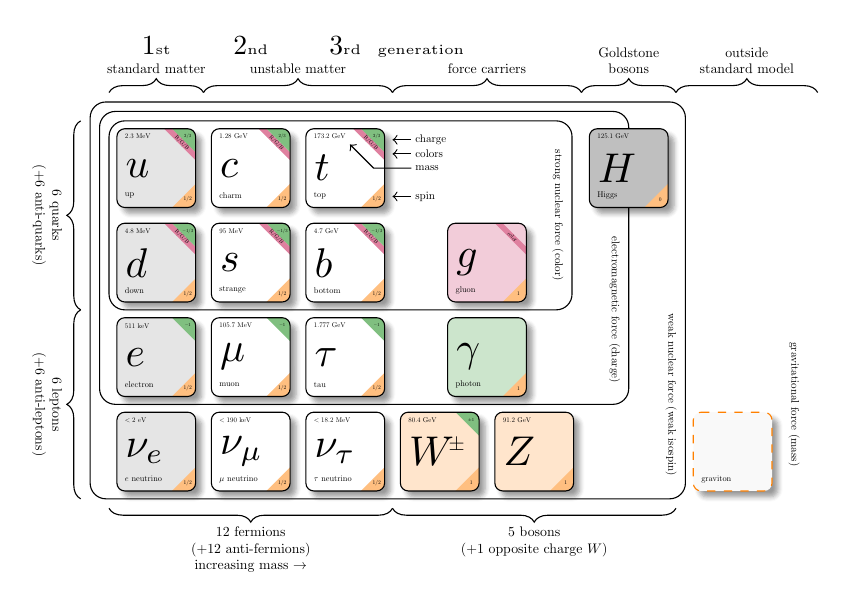
\begin{tikzpicture}[x=1.2cm, y=1.2cm]
  % draw force blocks
  \draw[round] (-0.5,0.5) rectangle (4.4,-1.5);     % strong force
  \draw[round] (-0.6,0.6) rectangle (5.0,-2.5);     % electromagnetic force
  \draw[round] (-0.7,0.7) rectangle (5.6,-3.5);     % weak force

  % draw all particles  
  \node at(0, 0)   {\particle[gray!20!white]
                   {$u$}        {up}       {$2.3$ MeV}{1/2}{$2/3$}{R/G/B}};
  \node at(0,-1)   {\particle[gray!20!white]
                   {$d$}        {down}    {$4.8$ MeV}{1/2}{$-1/3$}{R/G/B}};
  \node at(0,-2)   {\particle[gray!20!white]
                   {$e$}        {electron}       {$511$ keV}{1/2}{$-1$}{}};
  \node at(0,-3)   {\particle[gray!20!white]
                   {$\nu_e$}    {$e$ neutrino}         {$<2$ eV}{1/2}{}{}};
  \node at(1, 0)   {\particle
                   {$c$}        {charm}   {$1.28$ GeV}{1/2}{$2/3$}{R/G/B}};
  \node at(1,-1)   {\particle 
                   {$s$}        {strange}  {$95$ MeV}{1/2}{$-1/3$}{R/G/B}};
  \node at(1,-2)   {\particle
                   {$\mu$}      {muon}         {$105.7$ MeV}{1/2}{$-1$}{}};
  \node at(1,-3)   {\particle
                   {$\nu_\mu$}  {$\mu$ neutrino}    {$<190$ keV}{1/2}{}{}};
  \node at(2, 0)   {\particle
                   {$t$}        {top}    {$173.2$ GeV}{1/2}{$2/3$}{R/G/B}};
  \node at(2,-1)   {\particle
                   {$b$}        {bottom}  {$4.7$ GeV}{1/2}{$-1/3$}{R/G/B}};
  \node at(2,-2)   {\particle
                   {$\tau$}     {tau}          {$1.777$ GeV}{1/2}{$-1$}{}};
  \node at(2,-3)   {\particle
                   {$\nu_\tau$} {$\tau$ neutrino}  {$<18.2$ MeV}{1/2}{}{}};
  \node at(3,-3)   {\particle[orange!20!white]
                   {$W^{\hspace{-.3ex}\scalebox{.5}{$\pm$}}$}               
                                {}              {$80.4$ GeV}{1}{$\pm1$}{}}; % W
  \node at(4,-3)   {\particle[orange!20!white]
                   {$Z$}        {}                    {$91.2$ GeV}{1}{}{}}; % Z
  \node at(3.5,-2) {\particle[green!50!black!20]
                   {$\gamma$}   {photon}                        {}{1}{}{}}; % gamma-photon
  \node at(3.5,-1) {\particle[purple!20!white]
                   {$g$}        {gluon}                    {}{1}{}{color}}; % g-gluon
  \node at(5,0)    {\particle[gray!50!white]
                   {$H$}        {Higgs}              {$125.1$ GeV}{0}{}{}}; % H-Higgs
  \node at(6.1,-3) {\particle[gray!5!white]
                   {}           {graviton}                       {}{}{}{}}; % graviton

  % add text labels for forces
  \node at(4.25,-0.5) [force]      {strong nuclear force (color)};
  \node at(4.85,-1.5) [force]    {electromagnetic force (charge)};
  \node at(5.45,-2.4) [force] {weak nuclear force (weak isospin)};
  \node at(6.75,-2.5) [force]        {gravitational force (mass)};

  % draw arrows and add labels for legends
  \draw [<-] (2.50,0.30)  -- (2.7,0.3)          node [legend] {charge};
  \draw [<-] (2.50,0.15)  -- (2.7,0.15)         node [legend] {colors};
  \draw [<-] (2.05,0.25)  -- (2.3,0) -- (2.7,0) node [legend]   {mass};
  \draw [<-] (2.50,-0.3)  -- (2.7,-0.3)         node [legend]   {spin};

  % draw vertical braces and labels
  \draw [mbrace] (-0.8,0.5)  -- (-0.8,-1.5)
                 node[leftlabel] {6 quarks\\(+6 anti-quarks)};
  \draw [mbrace] (-0.8,-1.5) -- (-0.8,-3.5)
                 node[leftlabel] {6 leptons\\(+6 anti-leptons)};
  % draw bottom braces and labels                  
  \draw [mbrace] (-0.5,-3.6) -- (2.5,-3.6)
                 node[bottomlabel]
                 {12 fermions\\(+12 anti-fermions)\\increasing mass $\to$};
  \draw [mbrace] (2.5,-3.6) -- (5.5,-3.6)
                 node[bottomlabel] {5 bosons\\(+1 opposite charge $W$)};

  % draw top braces and add text labels
  \draw [brace] (-0.5,.8) -- (0.5,.8) node[toplabel]         {standard matter};
  \draw [brace] (0.5,.8)  -- (2.5,.8) node[toplabel]         {unstable matter};
  \draw [brace] (2.5,.8)  -- (4.5,.8) node[toplabel]          {force carriers};
  \draw [brace] (4.5,.8)  -- (5.5,.8) node[toplabel]       {Goldstone\\bosons};  % two lines
  \draw [brace] (5.5,.8)  -- (7,.8)   node[toplabel] {outside\\standard model};  % two lines

  % add big numbers on top
  \node at (0,1.2)   [generation] {1\tiny st};
  \node at (1,1.2)   [generation] {2\tiny nd};
  \node at (2,1.2)   [generation] {3\tiny rd};
  \node at (2.8,1.2) [generation] {\tiny generation};
\end{tikzpicture}
\end{document}
